\section{Weryfikacja}
Weryfikacja działania została przeprowadzona~przez~autora pracy~na~gotowej~do~ewaluacji wersji aplikacji. Jej celem było potwierdzenie poprawności działania mechanizmu zbierania danych oraz wyciągnięcie pierwszych wniosków~o~przydatności~i~działaniu narzędzia.

\subsection{Wskazanie popularności elementów}
Przegląd map cieplnych pozwala~na~łatwą identyfikację częściej~i~rzadziej używanych funkcji, ekranów~i~elementów interfejsu aplikacji. Szczególnie dobrze nadają się~do~tego celu mapy kumulacyjne elementów nawigacji. Testowana aplikacja posiada dolny pasek nawigacji dzielący~ją~na~trzy obszary: panel, plany oraz nagrody. Na~poniższej mapie można zauważyć~że~pierwsza zakładka jest używana najczęściej podczas gdy pozostałe dwie~są~wybierane~przez~użytkowników~w~przybliżeniu~tak~samo często.

\bigskip
\img{\chapterPath/[bottom-nav-bar].png}{Pasek nawigacji testowanej aplikacji}{rs_bottom_nav_bar}{.7}

\subsection{Ekrany~i~obszary przewijane}
Ekrany posiadające potencjalnie przewijane obszary muszą być rozdzielone~na~mapę interakcji~ze~statycznymi elementami interfejsu oraz mapę zawartości znajdującej się~w~przewijanym polu. Na~poniższych obrazkach przedstawiony jest przykład takiej sytuacji. Po~prawej stronie znajduje się mapa obszaru przewiniętego~przez~użytkownika. Można też wywnioskować~że~większość~z~zarejestrowanych dotknięć ekranu znajdujących się~w~pionowej osi centralnej ekranu była spowodowana jego przewijaniem. 

\bigskip
\begin{figure}[H]
\centering
\begin{minipage}{.35\textwidth}
	\centering
	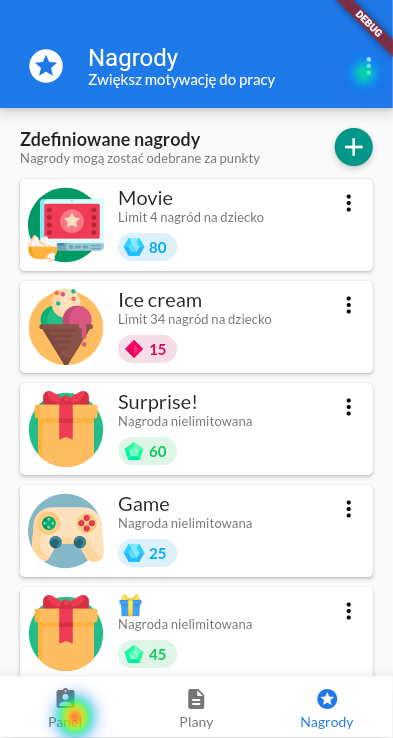
\includegraphics[width=.9\linewidth]{\chapterPath/caregiver-awards-page.png}
\end{minipage}
\begin{minipage}{.3\textwidth}
	\centering
	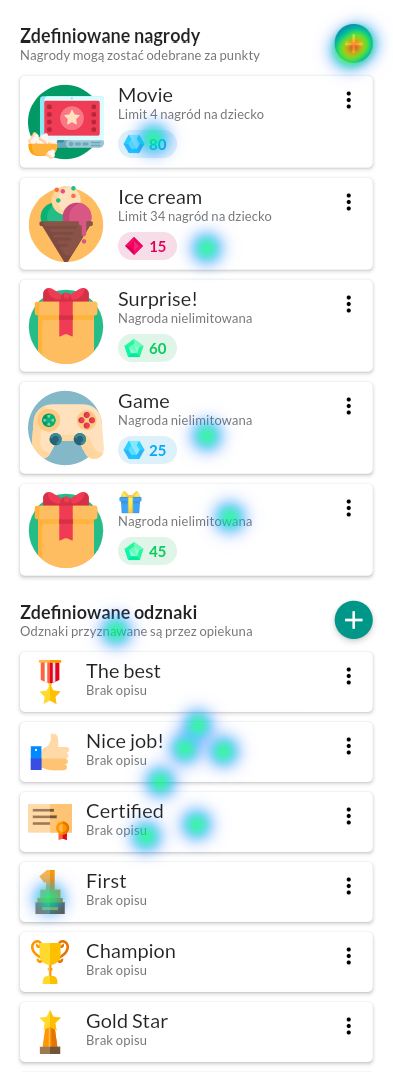
\includegraphics[width=.9\linewidth]{\chapterPath/[main-scroll-area] caregiver-awards-page.png}
\end{minipage}
\bigskip
\caption{Ekran nagród użytkownika}
\label{fig:rs_panel_parts}
\end{figure}

\subsection{Niewidoczne elementy}
Aktualnie~w~niektórych przypadkach,~na~przykład kiedy~w~aplikacji używany jest gotowy komponent, niemożliwe może być zawarcie~go~na~mapie cieplnej. Taki przypadek przedstawiony jest poniżej. Pomimo~że~w~aplikacji użytkownik wybiera ikonę nagrody~z~wysuwającej się~od~dołu karty,~na~mapie cieplnej karta~nie~jest widoczna mogąc powodować mylne zakwalifikowanie interakcji jako dotknięcia pustej przestrzeni~na~ekranie. To~aktualne ograniczenie zostało opisane jako jeden~z~punktów~w~sekcji \nameref{sec:future_work}.

\bigskip
\begin{figure}[H]
\centering
\begin{minipage}{.3\textwidth}
	\centering
	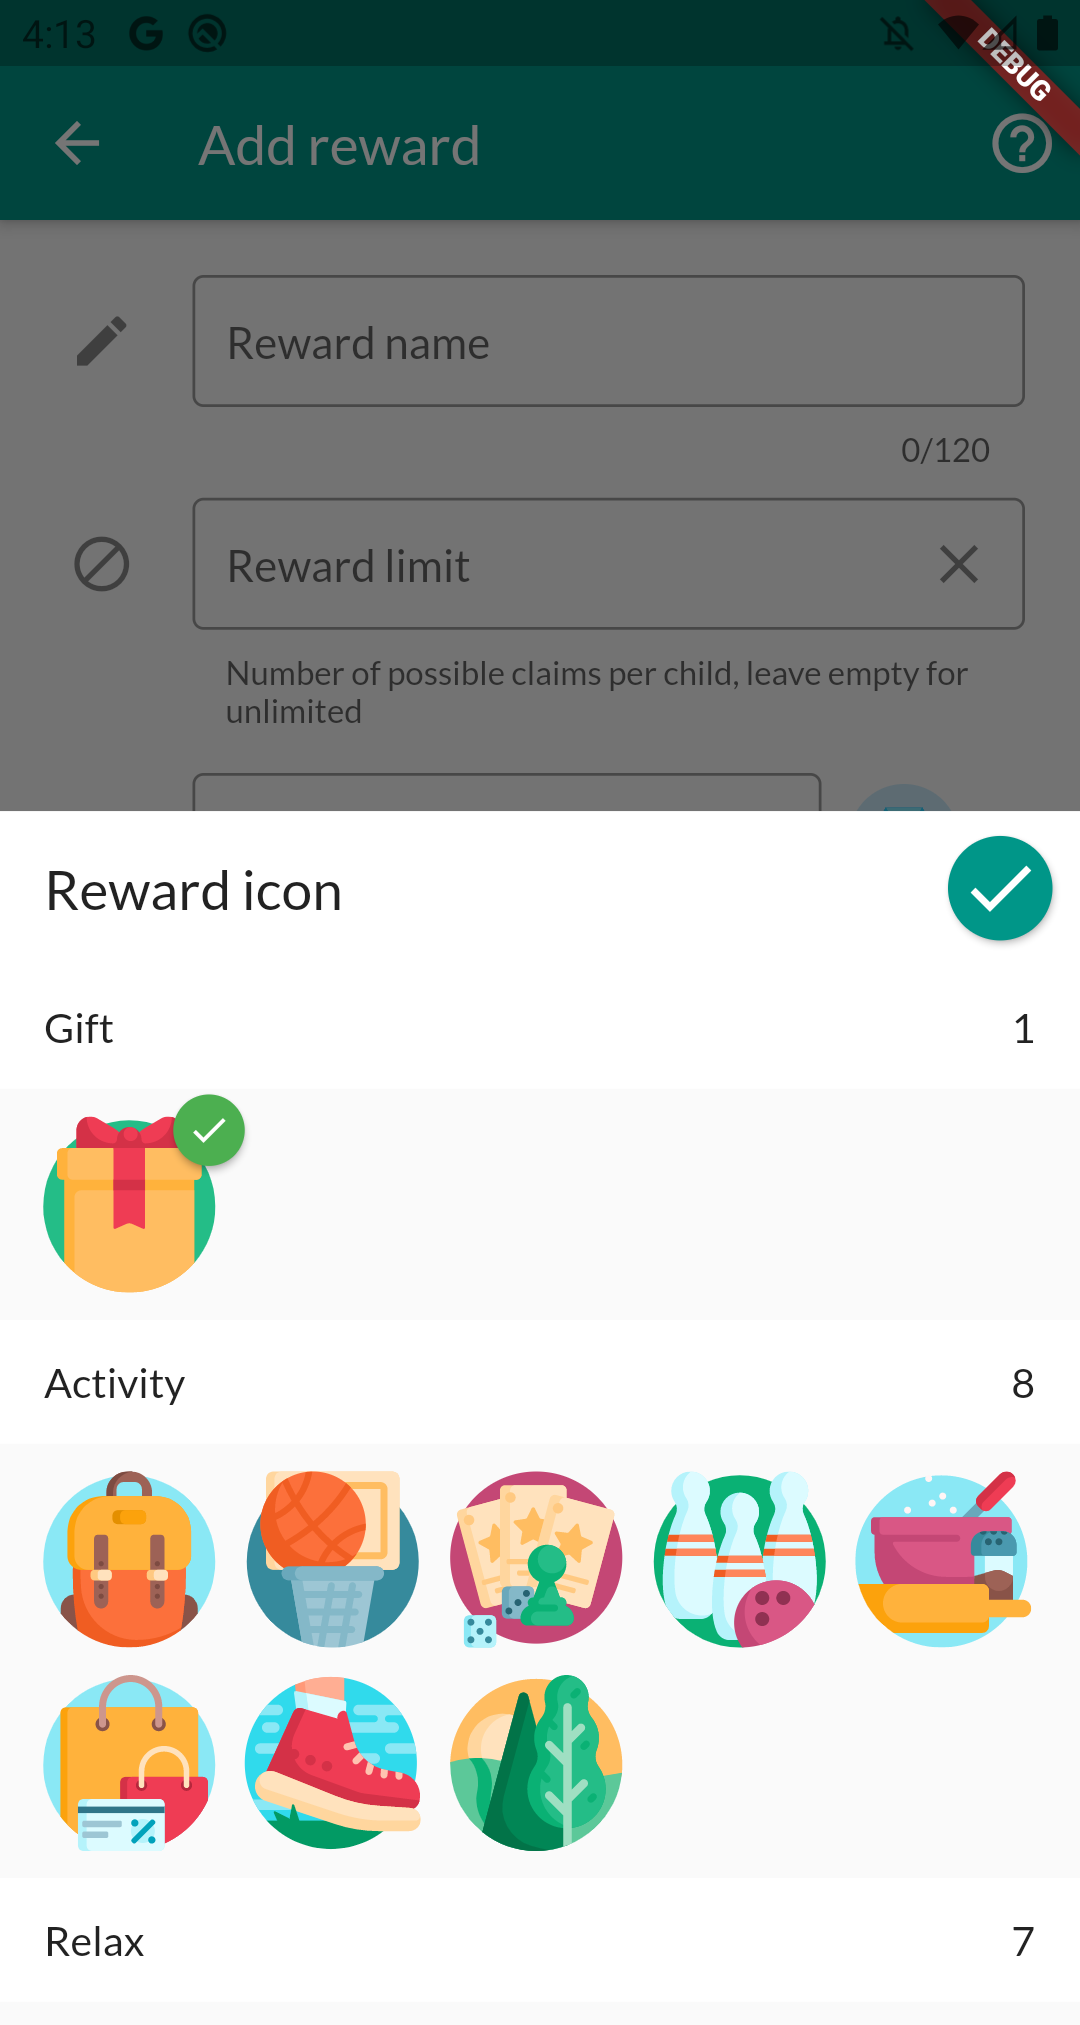
\includegraphics[width=.9\linewidth]{\chapterPath/smart-select-popup.png}
\end{minipage}
\begin{minipage}{.3\textwidth}
	\centering
	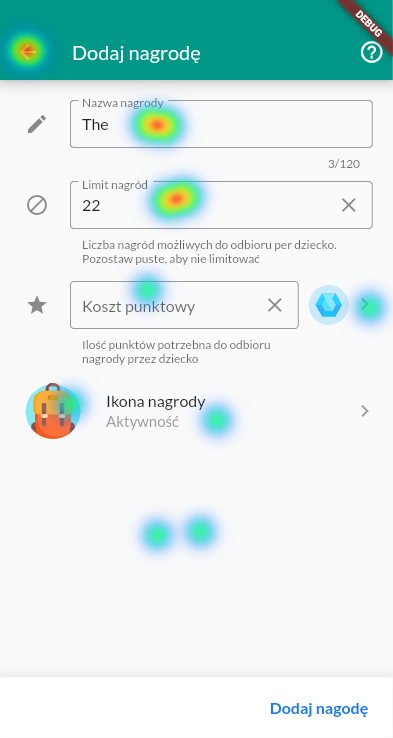
\includegraphics[width=.9\linewidth]{\chapterPath/caregiver-rewards-form-page.png}
\end{minipage}
\bigskip
\caption{Ekran tworzenia nagrody~i~powstała mapa cieplna}
\label{fig:rs_reward_form}
\end{figure}

\subsection{Zmienne elementy}
W przypadku przewijanych obszarów zawierających animowane (zmieniające zawartość, wielkość~lub~kształt) elementy, tło stworzonych map może~nie~być spójne. Wynika~to~z~opisanego już mechanizmu stopniowego tworzenia tła~z~części wyświetlanych~na~ekranie~w~danym momencie. W~poniższym przykładzie~po~lewej stronie widać widok kart~na~ekranie aplikacji. W~trakcie przewijania widok jest animowany powodując powiększenie aktualnie wyświetlanej~na~środku karty. Po~prawej stronie umieszczona została mapa cieplna złożona~z~trzech kart~po~ich przewinięciu~przez~użytkownika. Z~powodu połączenia obrazków~na~których~ta~sama karta~ma~różną wielkość obie boczne karty zawierają defekty graficzne. Pomimo tego ograniczenia wynikowe tło mapy cieplnej nadal spełnia swoją funkcję pozwalając~na~umiejscowienie interakcji użytkowników~na~ekranie.

\bigskip
\begin{figure}[H]
\begin{minipage}{.25\textwidth}
	\centering
	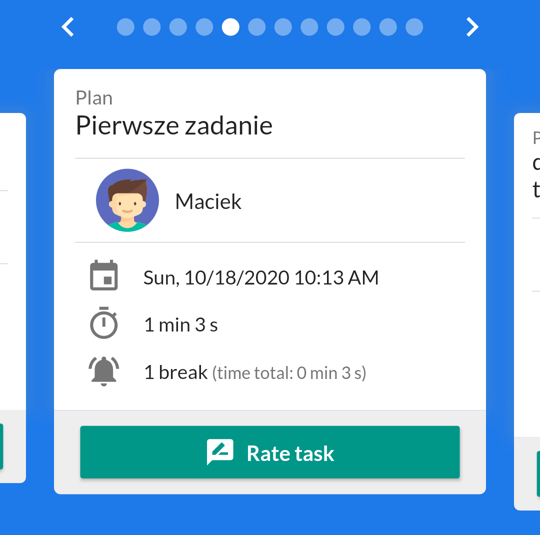
\includegraphics[width=.9\linewidth]{\chapterPath/rating_cards-app.png}
\end{minipage}
\begin{minipage}{.74\textwidth}
	\centering
	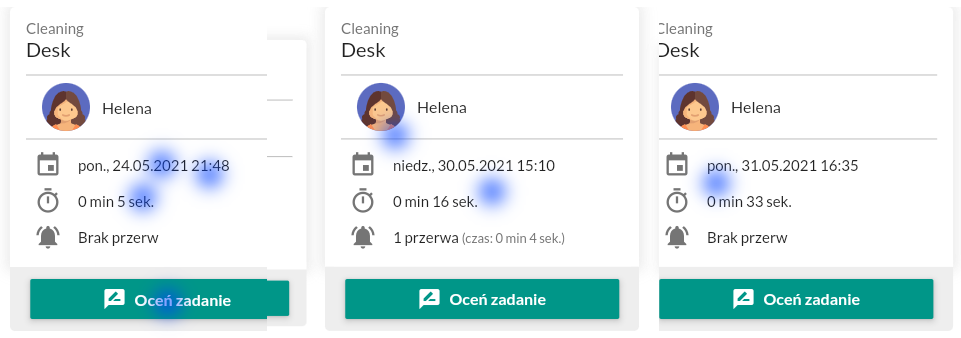
\includegraphics[width=.9\linewidth]{\chapterPath/[rating-cards]-caregiver-rating-page.png}
\end{minipage}
\bigskip
\caption{Widok kart~w~aplikacji oraz~na~mapie cieplnej}
\label{fig:rs_rating_cards}
\end{figure}
